\documentclass[a4paper, 12pt]{article}

\usepackage[T1]{fontenc}
\usepackage[utf8]{inputenc}
\usepackage[english]{babel}
%\usepackage[top=3cm,left=3cm]{geometry}

\usepackage{fancyhdr}  % page headers
\usepackage{graphicx}  % \includegraphics
\usepackage{xcolor}    % \definecolor
\usepackage{colortbl}  % for colouring tables
\usepackage{cite}      % \cite formatting
\usepackage{url}       % \hyperref, \url, \href
\usepackage{hyperref}  % references become hyperlinks
\usepackage{mathtools} % amsmath++
\usepackage{tikz}      % graphs
\usepackage{epsfig}    % .epsi graphics
\usepackage{subcaption}

\usepackage{microtype} % better linebreaking
\usepackage{eso-pic}   % alternative to ku-forside
%\usepackage{libertine} % nice regular font
\usepackage[scaled=0.9]{inconsolata} % nice teletype font
\usepackage{array}     % extensible array, tabular
%\usepackage{parskip}   % paragraphs

\usepackage{fancyvrb}  % Use verbatim as: !this!
\DefineShortVerb{\!}

%%%%%%%%%%%%%%%%%%%%%%%%%%%%%%%%%%%%%%%%%%%%%%%%%%%%%%%%%%%%%%%%%%%%%%%%
% Code excerpts
\usepackage{listings}

\definecolor{Brown}{cmyk}{0,0.81,1,0.60}
\definecolor{OliveGreen}{cmyk}{0.64,0,0.95,0.40}
\definecolor{CadetBlue}{cmyk}{0.62,0.57,0.23,0}
\definecolor{lightlightgray}{gray}{0.9}

\lstset{ %
  backgroundcolor=\color{lightlightgray},
  basicstyle=\scriptsize\ttfamily,
  breakatwhitespace=false,
  breaklines=false,
  language=matlab,
  deletekeywords={mean},
  morekeywords={rep, seq, rnorm, cbind},
  escapeinside={\%*}{*)}, % add LaTeX code inside code. example: val x%*$_1$*) = 42
  extendedchars=true,
  frame=none,
  numbers=left,
  numbersep=5pt,
  numberstyle=\tiny\color{gray},
  commentstyle=\color{gray},
  keywordstyle=\color{OliveGreen},
  showspaces=false,
  showstringspaces=false,
  showtabs=false,
  stepnumber=1,
  tabsize=4,
}
%%%%%%%%%%%%%%%%%%%%%%%%%%%%%%%%%%%%%%%%%%%%%%%%%%%%%%%%%%%%%%%%%%%%%%%%

%\setlength\parskip{1em}
%\setlength{\parindent}{0pt}
\def\arraystretch{2}

\newcommand{\shellcmd}[1]{\\\indent\indent\texttt{\footnotesize\# #1}\\}

\title{
  \vspace{5em}
  Principles of Computer Systems Design \\
  Final Exam
}

\author{%
  \begin{tabular}{l l l}
    Philip Munksgaard & 1989-07-24 & pmunksgaard@gmail.com
  \end{tabular}
}

\date{\today}

\begin{document}

\AddToShipoutPicture*{\put(0,0){\includegraphics*[viewport=0 0 700 600]{ku-farve}}}
\AddToShipoutPicture*{\put(0,602){\includegraphics*[viewport=0 600 700 1600]{ku-farve}}}
\AddToShipoutPicture*{\put(0,0){\includegraphics*{nat-en}}}

\clearpage
\maketitle

\thispagestyle{empty}

\newpage

\fancyhead[LO,RE]{Philip Munksgaard}
\fancyhead[LE,RO]{PCSD, Final Exam \\ \today }
\pagestyle{fancy}

\section*{Theory part}

\subsection*{Question 1 - Proximity}

We wish to examine the performance of an algorithm that merges two big
data sets $R$ and $S$ of $N_1$ and $N_2$ records, respectively, based
on comparison of a $k$ word key. Each record in either data set is $l$
words long. We assume that, by ``merge'', an actual merge-join
operation is the requested operation. We use $M$ to denote the amount
of memory available.

\subsubsection*{CPU Cost}

The data sets are very large, but let us assume that they aren't
larger than $M^2$, such that we can use two-phase merging
algorithms. Now, even though the data sets are (presumably) already in
some kind of database, we cannot reasonably expect them to be
pre-sorted. If that were the case, a simple merge-join would require
at most $(N_1 + N_2) \cdot k$ word comparisons to determine a merge of
the two data sets, as well as $\textrm{max}(N_1, N_2) \cdot (2l - k)$
CPU operations to write the data, since the merged records have size
$2l - k$. If they aren't sorted we can perform either a merge-join
where we first sort the two inputs, which gives an added cost of
$O(N_1 \cdot log(N_1) + N_2 \cdot log(N_2))$, or a hash-join. The
hash-join algorithm uses a hashing function to compute the hash value
for the key. Assuming it takes $h$ word operations to compute the
hash-function, we need to read and compute the hash function for each
relation, $h \cdot (N_1 + N_2)$; store the relations in buckets and
write those buckets to disk $l(N_1+N_2)$, before finally reading the
buckets from disk and joining them with a one-pass join, $l(N_1 +
N_2)$.

If the data sets are so large that we cant apply two-phase merging, we
have to use multi-phase merging. For a given intenger $d$, let us
consider $d$-way merging. For simplicity, we'll concentrate on the
merge-sort algorithm. Here, the difficulty is in sorting the data
sets. The idea is to take the two data sets $R$ and $S$, split them
into a number of groups, $N$, such that we can hold exactly $N+1$
blocks in memory at a time, and recursively sort them. When the groups
are sorted, merge them by reading one block from each group into
memory at at time. Sorting takes $O((N_1 + N_2) \cdot log_N(N_1 +
N_2))$ time, and merging is linear in the number of total records.

However, for these kinds of operations, the time spent by the CPU on
sorting, computing hash functions, merging and the like, is more or
less completely overshadowed by the cost of disk I/O.

\subsubsection*{I/O cost}

%% Analyse the I/O cost of this algorithm. Use B to denote the size of
%% the memory blocks (pages) transferred between the disk and main
%% memory and M to denote the size of main memory; both measured in
%% words.

Now we wish to examine the I/O cost of merging the data sets using a
$d$-phase merging algorithm. We let $B$ denote the page size (distinct
from the $B(\ldots)$ we use to denote the amount of pages something
occupies), and $M$ denote the size of main memory; both measured in
words.

First we need to figure out how many passes are needed to sort the
data sets into $(M-1)/B$ blocks. Using the algorithm described in
section 15.8.2 of \emph{Database Systems: The Complete Book}, we
simply run it with increasing values of $k$, until the result is
smaller than $M$. We get a number $k$, which is how many passes we
need to make. Then, we can simply use the calculations from that same
chapter, giving us a total of $(2d-1)(B(R) + B(S))$ disk I/O's, where
$B(R) = lN_1 / B$, meaning that $R$ takes up $lN_1$ words of space,
which is the same as $lN_1 / B$ pages, and analogously for $S$, just
using $N_2$ instead.

\subsubsection*{Address-translation cost}

%% Analyse the address-translation costs of this algorithm. Use W to
%% denote the size of the address- translation cache measured in words
%% and P to denote the branching factor of the nodes in the page
%% table.

We now wish to analyze the address-translation cost of this
algorithm. We will use $W$ to denote the size of the TLB measured in
entries (the assignment text says words, but in my opinion entries is
a much more meaningful metric, and translation between the two is
trivial, given a specific architecture) and $P$ to denote the
branching factor of the nodes in the page table tree.

First, let us consider the sorting phases. Each block is read into
memory once. For each word in the block, we have at least one
TLB-miss, meaning that we'll have to do a page-lookup, taking $O(d)$
time ($d$ being the height of the page table). For simplicity, we'll
assume that sorting is possible in a single pass. Then, by using a
depth-first search, we minimize the number of TLB-misses that occur:
when the size of each merge-group is less than $W$, we don't have any
more TLB-misses in that branch, giving us a rough estimate of
$O(n\cdot (log (n) - log(W))$ TLB-misses.

When merging the groups, we can expect an almost linear amount of
TLB-misses, since each head in the group only misses once, and,
assuming that $W$ is larger than the amount of groups, we can keep the
address of each head in the TLB until it is no longer used.

It should be noted though, that many advanced techniques of modern
processors invalidate or, at the very least, makes it hard to reason
about the address-translation costs of particular algorithms. For
example, memory prefetching makes it hard to predict how many misses
there will be, and the increasingly larger caches might completely
invalidate some concerns about cache misses.

\subsection*{Question 2 - Parallelism}

In this question, we examine the properties of a hash-join operations
for two big relations $R$ and $S$, with $N_R$ and $N_S$ records,
respectively, on a shared-nothing database system with $p$
processors. The algorithm uses two hash functions $h_1$ and $h_2$ to
partition records and map them to processors, respectively.

\subsubsection*{Hash function Domains and Ranges}

The function $h_1$ is used to partition the records of $R$ and $S$
into $k$ buckets each. That means, that $h_1$s domain is the key used
to compare the two relations, while its range is the numbers $1\cdots
k$. Similarly, $h_2$ is used to map the record buckets to processors,
which then join a pair of record buckets $R_i, S_i$. Therefore, the
domain of $h_2$ is the numbers $1 \cdots k$, while the range is the
numbers $1 \cdots p$.

\subsubsection*{Functional description}

The algorithm works by first using the hash function $h_1$, to
partition the input data in $R$ and $S$ into $k$ buckets each, such
that we have buckets $R_1, R_2, \ldots, R_k$ and $S_1, S_2, \dots,
S_k$. Each bucket is distributed out to one of the $p$ processors,
using the $h_2$ hashing function, such that, if $h_2(1) = 2$,
processor $p_2$ merges buckets $R_1$ and $S_1$. We expect $k<p$, such
that each processor has at least one bucket to merge. The merge is
then executed locally, using the techniques described in section 15.3
of \emph{Database Systems: The Complete Book}.

\begin{figure}
  \center
  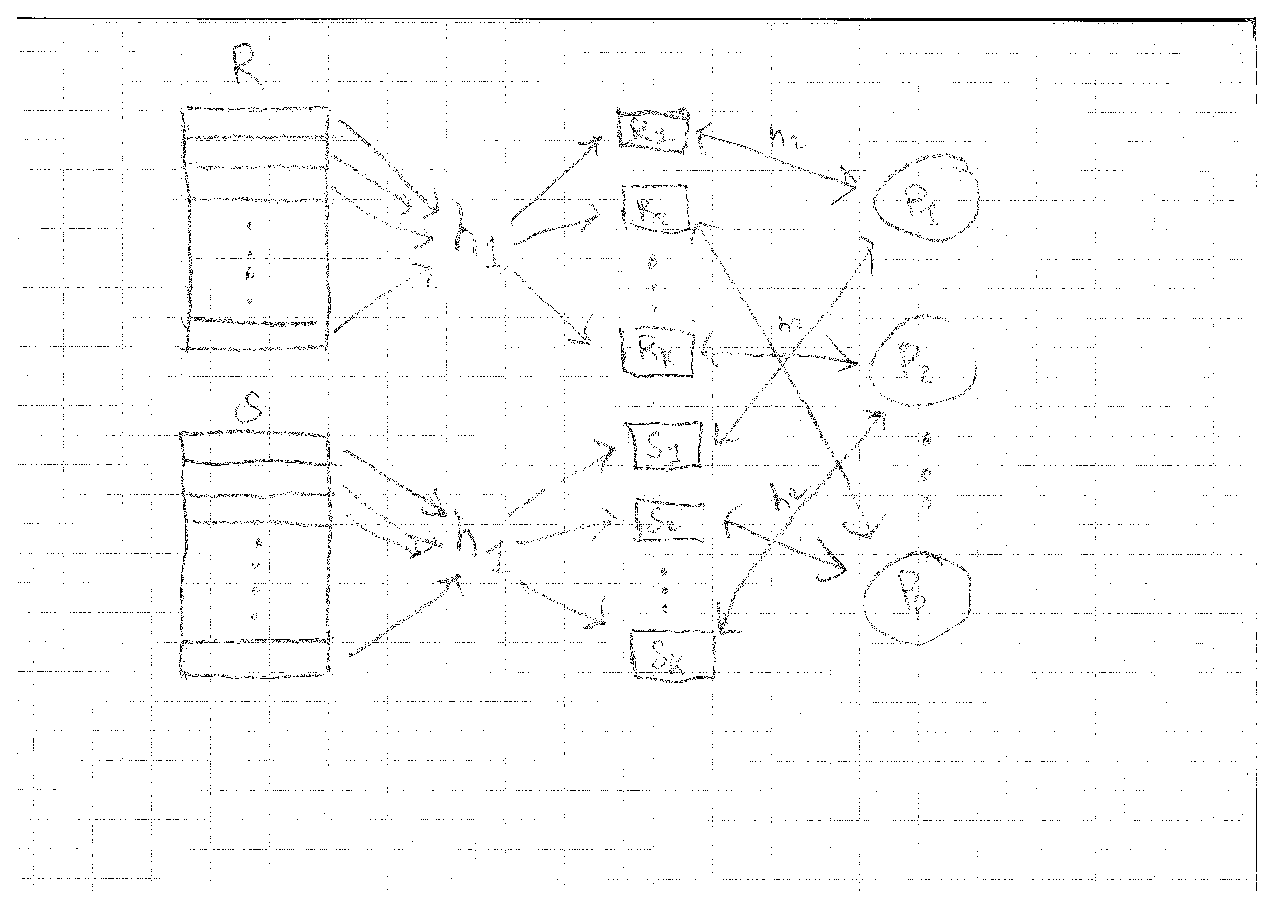
\includegraphics[scale=0.6]{parallelmerge.eps}
  \caption{Drawing, showing how the hash-functions, buckets and
    processors interact in our version of parallel hash-merge.}
\end{figure}

On a lower level, the initial partitioning could be performed by a
separate processor, which would immediately send the partitioned
groups to the corresponding merge processors. This way, we wont have
to worry about synchronization issues with regards to the
partitioning. For the purposes of this assignment, we will assume that
results are simply kept in memory at the merging processors, since we
don't know if they are supposed to be further processed, passed on or
simply stored. Taking the initial costs for such last steps into
account is a trivial matter (simply add one I/O write, or message pass
for each block), so we'll leave it out of any further computations.

\subsubsection*{I/O cost}

We wish to describe how many I/Os each processor performs. For the
purposes of this assignment, we'll assume uniform hashing, and that
the processors receive the partitioned groups from a separate
partitioning server.

First of all, for each pair of relations $R_i$, $S_i$ that a
particular processor has to merge we have to receive the whole bucket
before we can perform any merging. Hence, each processor, upon
receiving partitioned group blocks from the partitioning server, has
to write them to disk, until we know that all blocks have been
received. Assuming uniform hashing, that adds up to $(B(R) + B(S)) /
p$ writes, where $B(X)$ is the amount of blocks required to store the
relation $X$. Then, depending on the size of the processors memory, it
has to perform a single-pass merge or a multi-pass merge. Let's assume
that a two-pass merge is necessary. Using a normal merge-join or
hash-join uses $3(B(R) + B(S))$ disk I/Os, but given certain
circumstances (specifically, that the expected size of buckets isn't
too big), we could also employ the more effective \emph{hybrid
  hash-join}, which would give us $(3 - 2M/ B(S))(B(R) + B(S))$ disk
I/O.

\subsubsection*{Message cost}

Each processor only has to receive a message each time the
partitioning server has a full block: Each time that happens the
partitioning server simply sends the block and starts on a new one. If
the block size is $B$ and we assume uniform hashing, that means that
the partitioning server has to send $(B(R) + B(S)) / B$ messages in
total, which also means that each merging server receives $(B(R) +
B(S)) / pB$ messages.

For the purposes of this exercise, let's further assume that each
server has to pass the resulting merged relation on to another (disk)
server for storage. That would mean that, in addition to the messages
received as described above, each server also has to send the merged
relations. Doing so requires another $\textrm{max}(N_R, N_S) / (F(R,
S) \cdot p)$ messages, where $F(R,S)$ is the size in blocks of a
merged relation (more concretely, if we're given the two relations
$R(X,Y)$ and $S(Y,Z)$, $F(R,S)$ is the size of the resulting joined
relation $T(X,Y,Z)$).

\section*{Programming Part}

\subsection*{Question 1 - Implementation}

%% Overall implementation of OrderManager and ItemSupplier, including
%% the following:

%% - Considering your use of logging, what RPC semantics are
%% effectively implemented between clients and OrderManager or
%% ItemSupplier? What RPC semantics are effectively implemented
%% between OrderManager and ItemSupplier? Explain.

%% - How did you make workflow processing asynchronous at the
%% OrderManager?

The !CertainItemSupplier! class is the basic !ItemSupplier!
implementation. Its constructor is called with a supplier ID and set
of valid item IDs. It is assumed that each !CertainItemSupplier! has a
fixed list of valid item IDs that it can supply. Any requests for
other item IDs will result in an !InvalidItemException! being
thrown. Apart from the !InvaliIdtemException!, we've also implemented
a number of other subexceptions to !OrderProcessingException!, that
make communication and error handling easier.

The !executeStep! method ensures \emph{all-or-nothing atomicity} by
first making sure that all steps have the correct supplier ID, and
that all item IDs are available at that supplier, and finally that the
amount requested is a positive number (it does not make sense to order
zero or a negative number of items). As the !getOrdersPerItem! method
does not modify any data, we are not concerned with all-or-nothing
atomicity; we just have verify that the item IDs are valid before
querying for the amounts.

The !CertainItemSupplier! class also contains a read-write lock, which
is used to ensure before-or-after atomicity of the operations on the
same item supplier: In !executeStep!, the write-lock is acquired after
verifying the supplier and item IDs; in !getOrdersPerItem! it is
acquired after we've verified the item IDs. This ensures
before-or-after atomicity in !CertainItemSupplier!.

Another approach would have been to have individual read-write locks
for each item ID in the item supplier. However, for simplicity and
ease-of-reasoning, we chose to have just one global lock per item
supplier. We assume that, for this system, !executeStep!, and
therefore modifying updates, will be called much more often than
!getOrdersPerItem! (I feel bad for the item supplier where the
opposite is true), so in either case, the locks acquired will most
likely be exclusive ones. For item suppliers which provide many item
IDs and where most incoming orders only request a few different item,
(say, each order only requests 10 different items, and the supplier
has a thousand different items), we expect a much higher latency using
our method, but if each item supplier only has a small amount of
different items, the benefits of the global-lock approach (that is,
not having to acquire $n$ different locks for $n$ items) far outweigh
the benefits of locking each individual item.

The item supplier is then made available to clients via an RPC
interface that uses HTTP to transfer request and response objects over
the network, which is implemented in the !ItemSupplierHTTPServer! and
related classes. The HTTP server is called by running the
!startServer! method, supplying a port number, a supplier ID and a set
of valid item IDs~\footnote{It is also possible to run the main method
  from the command-line, simply supply port number, supplier ID and a
  number of valid item IDs. } . Clients then use the
!ItemSupplierProxy! class to interface with the item supplier. That
class is called with an address (``http://127.0.0.1:8080'', for
example) and a corresponding supplier ID. This means that each proxy
only handles communication with a single item supplier.

\paragraph{}

The !CertainOrderManager! class is the basic !OrderManager!
implementation. Its constructor is called with a manager ID and a map
containing ItemSuppliers mapped by their IDs.

The !registerOrderWorkflow! method executes the workflow
asynchronously by launching a special !Worker! class in a separate
thread. The !Worker! class is supplied with a !Workflow!, a simple
container class for data pertaining to a work flow, and tries to run
the steps. All steps are continually tried until they succeed, except
if some unrecoverable error occurs, such as requesting an invalid item
or supplier ID, an invalid quantity or a malformed request. When a
step is successful or failed, the thread writes to a shared !Workflow!
object, which can be queried through the !getOrderWorkflowStatus!
method of !CertainOrderManager!. Another approach would have been to
spawn separate workers for each step of the workflow, but we opted for
this approach instead, since spawning threads can have considerable
overhead.

Since we can assume, cf. the
assignment handout, that we always either get a response from the item
supplier, or that the item supplier actually failed, we are thus using
\emph{at-most-once} RPC semantics between the order manager and item
supplier.

\paragraph{}

Durability is achieved by logging all incoming requests to the
!CertainOrderManager! and !CertainItemSupplier! classes. For these
purposes, a !Logger! class has been implemented. It has a !log! method
(which is !synchronized! in order to avoid interleaving outputs) that
is used to serialize an object to XML and write it to a file on
disk. Each !CertainOrderManager! and !CertainItemSupplier! has a
unique ID that is used to name a log file. For the
!CertainItemSupplier!, the log simply consists of all the !OrderStep!
objects that the !executeStep! method has received: The objects are
simply serialized into XML and appended to the log file (which is
flushed before returning). Similarly for the !List<OrderStep>! objects
that !registerOrderWorkflow! receives. This way, durability is
ensured, and recovery is as simple as reading the requests from the
log and executing them. It should be noted that, for the purposes of
this assignment, any already existing log files are deleted when
starting the !Logger!. Adapting the !CertainItemSupplier! and
!CertainOrderManager! classes to check for and recover from
preexisting log files, however, is a trivial matter.

\paragraph{}

%% - How did you handle failures of individual components? In
%% particular, how do you handle failure propagation?

Failure of an item supplier only affects those !OrderStep!s that are
directed towards that item supplier. As described above, the !Worker!
class will simply keep trying to execute the step
indefinitely. Exceptions at the item supplier is communicated through
the !ItemSupplierResponse! class (along with all the other relevant
response information), so the worker always knows if, for example it
has supplied an invalid item ID, or similar.

\subsection*{Question 2}

%% An ItemSupplier executes operations originated at multiple
%% instances of OrderManager as well as local clients. Describe how
%% you ensured atomocity of the operations. Mention the following:

%% Which method did you use to ensure serializability at each item
%% supplier?

%% Argue for the correctness of your method.

%% Argue for the performance of your model.

As discussed above, a simple global-locking mechanism is used in the
!CertainItemSupplier! class to ensure atomicity. As such,
serializability is trivially achieved, as is correctness. However, as
pointed out above, it also has certain drawbacks for some specific use
cases. Our method also ensures that deadlocks cannot occur, although
there is a slight possibility of starvation. However, as described
earlier, in a system like this, we expect far more order registrations
than order overview requests (for instance, we might expect suppliers
to execute !getOrdersPerItem! just a few times per day, in order to
figure out what to produce, package and send, whereas many hundreds or
thousands of customers might issue order registrations each day), so
the exclusive locks wont likely be starved by shared locks.

As mentioned, the alternative would be to have one lock for each item,
which could also quite easily be done, but the benefits of increased
concurrency might be offset by the large overhead of having to acquire
many different locks each time an order request is
issued. We would also have to take deadlocks into account, but they
can be quite easily prevented by first sorting the locks requested.

\subsection*{Question 3}

%% How would you recover from a failure of an OrderManager or an
%% ItemSupplier? For each of the two scenarios, explain necessary
%% interaction with other components to archieve recovery, how you
%% would use the log, why it is sufficient.

Recovery for both the !CertainOrderManager! and the
!CertainItemSupplier! is done by reading the log produced by the
!Logger! class. Since they are the only implementations of their
respective interfaces that actually do any work, they are the only
ones who need to log and recover data. As described above, the output
to the log simply consists of serialized versions of all incoming
requests. Thus, recovering is simply a matter of reading and executing
all the requests from the log in question.

Failures of the !OrderManager! servers should be handled by the
clients. Simply trying another server, or retrying the same server
should suffice. Similarly, and as mentioned above, the !Worker!
threads that !CertainOrderManager! uses to facilitate execution of
steps on item suppliers, simply keeps retrying until they get a
connection to their corresponding server.


\subsection*{Question 4}

%% Describe your high-level strategy to test your
%% implementation. Mention the following:

%% How you tested execution workflows by the OrderManager, considering
%% asynchronicity of execution.

%% How you tested operations were atomic at the ItemSupplier

%% How you tested error conditions and failures of multiple comonents.

The main testing takes part in the two classes !ItemSupplierTest! and
!OrderManagerTest!, which are part of the !test! subpackage of
!com.acertainsupplychain!.

The !ItemSupplierTest! tests the main functionality of the
!CertainItemSupplier! class. It does not use the RPC interface, but
instead it directly tests some of the business logic of the item
supplier. After building the entire project (by running
``\texttt{make}''), running it is a simple matter of executing the
command ``\texttt{ItemSupplierTest}''. It tests the
different error conditions that we expect from !CertainItemSupplier!,
as well as atomicity and isolation (which is tested by spamming the
item supplier from two different threads).

The !OrderManagerTest! is not quite as comprehensive, but tests the
entire RPC infrastructure, and that execution of workflows is indeed
done asynchronously. Running it is a bit more complex, as it requires
correctly configured and running instances of !OrderManagerHTTPServer!
and !ItemSupplierHTTPServer!. To start, run ``\texttt{make
  TestServer1}'' and ``\texttt{make TestServer2}'' in separate shells,
then run ``\texttt{make OrderManagerTest}'' in a third shell.

Testing for error conditions is covered by the tests mentioned
previously. However, one bit that we haven't touched on, is failure
and recovery when servers go down. However, it is easy to run the
!OrderManagerTest! in such a way that it demonstrates the order
managers ability to keep retrying requests when encountering
recoverable failures. Simply omit starting the
!ItemSupplierHTTPServer! before running the !OrderManagerTest!. You
should see a lot of error messages in the !OrderManagerHTTPServer!
window (these are output by the jetty client, with no apparent way to
turn them off...), but starting the !ItemSupplierHTTPServer! should
make them stop, and make the test proceed as usual.

As mentioned earlier, clients have to handle server failures
themselves, so running the !OrderManagerTest! without a running
!OrderManagerHTTPServer! will result in exceptions. However, they can
quite easily be handled, as has been done in !CertainOrderManager!
(which is essentially a acting as a client to an item supplier proxy).


\subsection*{Question 5}

%% Design, describe and execute an experiment that shows how your
%% implementation of a single ItemSupplier behaves as concurrency is
%% increased. Mention: Setup, Results. Also figures.

Performance experiments takes place in the
!com.acertainsupplychain.performance! package. Running the
!PerformanceTest! classe (optionally tweaking the !numlocalthreads!
and !numremotethreads! parameters first) will run the performance
tests against a running set of servers. To simplify, running
\texttt{make performance} runs the appropriate servers (remember to
kill them afterwards with \texttt{kill java}).

\subsection*{Setup}

The experiment took place on a laptop with the following
specifications: Intel i5 @ 4$\times$2.6GHz, 12GB RAM.

To carry out the experiments, one item supplier server is run, and
initialized with 100 items (consecutively numbered from 0 to 99, for
simplicity). A number of local and remote clients (using
!ItemSupplierProxy! and !OrderManagerProxy! respectively) then perform
some work on the item supplier.

Each worker runs for 200 warm up operations, followed by the actual
500 operations used in measurements. The local worker issues 10\%
!getOrdersPerItem! requests and 90\% !executeStep! requests. This is
supposed to mimic a situation where the local worker issues a lot of
requests, but only checks how many orders have been received a few
times per day. Similarly for the remote worker, which issues 40\%
!registerOrderWorkflow! requests and 60\% !getOrderWorkflowStatus!
requests. We assume that, once customers have ordered their items,
they'll have a tendency to check the order status a couple of times,
to figure out whether or not they are successful. Each operation uses
a randomly generated data set. For the purposes of this test, we are
always using the same number of local and remote clients, meaning that
if there are 20 total clients, 10 of those will be remote and the
remaining 10 local.

\subsection*{Results}

Our experiments show that the item suppliers throughput scales
somewhat well with the amount of clients, but also that latency
generally goes up, the more clients we have. The fact that throughput
generally rises with the amount of clients (at least for the
measurements we've performed) indicate that the local computations
performed by the item supplier isn't yet a major hurdle. Of course, at
some point, throughput is going to drop off, when the time spent
waiting for I/O is overcome by the time required to computing on the
server. However, since the computations performed by the item supplier
are relatively benign, we expect throughput to be able to climb for a
while. However, while throughput may rise, latency is almost
definitely going go up, the more clients we use. At some point, it
would be preferable to implement some kind of caching, or even
server replication, in order to bring general latency down.


\begin{figure}
  \center 
  \includegraphics[scale=0.6]{throughput.eps}
  \caption{Throughput for the item supplier.}
\end{figure}

\begin{figure}
  \center
  \includegraphics[scale=0.6]{latency.eps}
  \caption{Latency for the item supplier.}
\end{figure}

\end{document}
